\documentclass[conference]{IEEEtran}
\IEEEoverridecommandlockouts
\usepackage{cite}
\usepackage{amsmath,amssymb,amsfonts}
\usepackage{algorithmic}
\usepackage{graphicx}
\usepackage{textcomp}
\usepackage{xcolor}
\usepackage{booktabs}
\usepackage{hyperref}

\def\BibTeX{{\rm B\kern-.05em{\sc i\kern-.025em b}\kern-.08em
    T\kern-.1667em\lower.7ex\hbox{E}\kern-.125emX}}
\begin{document}

\title{An Explainable and Sequence-Preserving BERT-BiLSTM Framework for Online Recruitment Fraud Detection}

\author{\IEEEauthorblockN{Akhilesh}
\IEEEauthorblockA{\textit{Department of Computer Science and Engineering} \\
\textit{M.Sc. (Data Science)}\\
India \\
email@example.com}
}

\maketitle

\begin{abstract}
Online recruitment platforms streamline candidate searches but also allow scammers to publish fraudulent job posts. These fake postings aim to steal personal identification details or extract illicit fees from job seekers. Manual inspection of job ads is slow and difficult because scammers copy legitimate company profiles. Traditional machine learning models fail to capture semantic context, while standard transformer architectures discard intermediate sequential structure by relying solely on a single classification vector. This paper presents an explainable, sequence-preserving hybrid framework combining Bidirectional Encoder Representations from Transformers (BERT) and a 2-layer Bidirectional Long Short-Term Memory (Bi-LSTM) network. The model fine-tunes bert-base-uncased to extract context-rich token hidden states, which are then passed to a 2-layer Bi-LSTM to retain sequential syntax. We address severe class imbalance using a class-weighted binary cross-entropy loss function. Furthermore, we integrate SHAP (SHapley Additive exPlanations) for token-level visual explainability, resolving the black-box limitation of deep networks. Evaluated on the EMSCAD dataset, the proposed model achieves a classification accuracy of 99.02\%, a Class 1 (Fraudulent) precision of 94.23\%, recall of 84.97\%, F1-score of 89.36\%, a macro-averaged F1-score of 94.42\%, and a ROC-AUC of 99.02\%. This setup outperforms the published Fraud-BERT baseline across all evaluated metrics and provides a transparent classification pipeline.
\end{abstract}

\begin{IEEEkeywords}
Online Recruitment Fraud, Fake Job Detection, Transformers, BERT, Bi-LSTM, Explainable AI, SHAP.
\end{IEEEkeywords}

\section{Introduction}
Online job portals like LinkedIn and Indeed have simplified recruitment, allowing companies to post job openings and connect with applicants quickly. However, these open platforms are vulnerable to Online Recruitment Fraud (ORF) \cite{taneja2025fraud}, \cite{pillai2023detecting}. Scammers publish fake job listings to obtain sensitive applicant data, such as national identification numbers and banking credentials, or to demand advance fees for visas, training, or equipment \cite{naude2023machine}. Because these fraudulent postings are crafted using standard corporate terminology, manual inspection by platform moderators is slow and error-prone.

Identifying these listings automatically requires natural language processing models capable of recognizing deceptive language. Early approaches used machine learning models like Logistic Regression and Random Forest \cite{chiraratanasopha2022detecting}. These models rely on TF-IDF or Bag-of-Words features, which produce sparse vectors that ignore word order and semantic context. Deep learning models, such as standard LSTMs and GRUs, capture sequence information but often use static embeddings like Word2Vec \cite{pillai2023detecting}. Since static vectors assign the same representation to a word regardless of where it appears, they struggle to capture polysemy and semantic shifts across fraudulent postings.

Pre-trained transformer models, particularly BERT, resolved context representation issues \cite{sanisetty2025comprehensive}, \cite{srilakshmi2026transformer}. BERT uses bidirectional self-attention to generate context-aware token representations. However, standard BERT classifiers pass only the classification token (\texttt{[CLS]}) to the output layer, discarding token-level sequential and contextual details across the text. Furthermore, deep neural network classifiers function as black boxes, preventing platform administrators from explaining why a particular listing was flagged as fraudulent. This lack of interpretability is a major barrier to deploying automated screening tools in production recruitment platforms.

To resolve these limitations, we propose a hybrid \textbf{BERT-BiLSTM} framework. Our approach uses a fine-tuned \textbf{bert-base-uncased} model to extract context-rich token embeddings. Instead of discarding the sequence, we feed the full sequence hidden states to a \textbf{2-layer Bidirectional LSTM (Bi-LSTM)} network to analyze sequential syntax and long-range word relationships. To address the class imbalance of the EMSCAD dataset (where fake ads constitute less than 5\% of postings), we apply a class-weighted loss function. Crucially, we integrate \textbf{SHAP (SHapley Additive exPlanations)} to extract token attributions, providing complete transparency by showing which words contribute to flagging a job as fake. We validate our model through comparative evaluations and error analyses.

In this work, we outline several contributions. First, we implement a robust preprocessing and concatenation pipeline that combines 10 metadata fields while filtering out null entries and formatting noise. Second, we present a sequence-preserving BERT-BiLSTM architecture that maintains token-level contextual hidden states. Third, we integrate SHAP for token-level visual explainability, addressing the black-box limitation. Finally, we provide a comprehensive empirical evaluation against multiple baselines, detailing class-specific, macro-averaged, and weighted-average classification metrics.

\section{Related Work}
Online recruitment fraud detection has received substantial attention as the number of online job boards has expanded. Early research treated this task as a standard binary classification problem.

\subsection{Machine Learning Approaches}
Salloum et al. \cite{salloum2024analysis} applied Logistic Regression and Decision Trees using TF-IDF feature extraction on job texts, achieving an accuracy of 96.78\%. However, their evaluation showed high variance in F1-scores, heavily biased toward the majority (genuine) class due to severe data imbalance. Chiraratanasopha and Chay-intr \cite{chiraratanasopha2022detecting} addressed this limitation by designing custom metadata features reflecting real-world fraud indicators, such as missing company logos, absence of screening questions, and specific salary exaggerations, which yielded an accuracy of 97.64\%. Naud{\'e} et al. \cite{naude2023machine} classified fraudulent job postings into specific sub-categories, demonstrating that Gradient Boosting classifiers using POS tags and rule-set features obtained an F1-score of 0.88. Additionally, Habib et al. \cite{habib2021fake} developed an ensemble voting classifier that integrates Random Forest and Naive Bayes to identify job vacancy fraud, showing notable stability on imbalanced sets. Roy et al. \cite{roy2020fake} benchmarked several traditional ML models and noted that Support Vector Machines (SVM) could extract reliable linear decision boundaries on smaller token vocabularies.

\subsection{Deep Learning and Transformer Models}
To overcome the sparsity of TF-IDF representations, deep learning models were introduced. Pillai \cite{pillai2023detecting} utilized a Bi-LSTM model trained on static word embeddings to capture temporal sequences in job text. While achieving a high accuracy of 98.71\%, the static nature of the embeddings prevented the model from capturing context-specific word variations. Alghamdi and Alharby \cite{alghamdi2019online} proposed Gated Recurrent Units (GRU) for identifying ORF scams, concluding that GRUs have fewer parameters than LSTMs while achieving similar classification capacity. Kumar and Garg \cite{kumar2022deceptive} investigated deceptive content detection on recruitment platforms using ensemble learning combined with Word2Vec representations. Vidros et al. \cite{vidros2017online} presented a systematic review and classification scheme for ORF, outlining standard guidelines for deep learning architectures in this domain.

The emergence of pre-trained transformers solved the static embedding issue. Taneja et al. \cite{taneja2025fraud} proposed \textit{Fraud-BERT}, fine-tuning a BERT classifier on the EMSCAD dataset and reporting a macro F1-score of 0.93 and accuracy of 99\%. Similarly, Sanisetty et al. \cite{sanisetty2025comprehensive} combined BERT with sentiment polarity analysis to model the emotional tone of descriptions. Gupta and Rani \cite{gupta2021contextualized} utilized contextualized representations from BERT to detect scams, reporting that bidirectional self-attention is extremely critical to capturing vocabulary variations. Liao and Wang \cite{liao2023online} recently combined a pre-trained transformer with a hybrid deep learning classifier to detect ORF, showcasing the benefits of feature extraction.

More recently, hybrid frameworks have been explored. Srilakshmi et al. \cite{srilakshmi2026transformer} and Varshitha et al. \cite{varshitha2026online} proposed architectures combining BERT/RoBERTa with a 2D Convolutional Neural Network (CNN2D) classifier, using oversampling methods to mitigate dataset imbalance. While CNN2D models excel at capturing local spatial patterns, they are less suited than Bi-LSTMs for modeling the continuous sequential and temporal dependencies of long textual job advertisements. Our research improves upon these existing models by pairing BERT's contextual power with a sequential Bi-LSTM head, offering a unified, computationally efficient framework that trains directly on the class-weighted imbalanced dataset without distorting original textual distributions.

\section{Proposed Methodology}
The proposed hybrid BERT-BiLSTM framework consists of four main steps: (A) Robust Concatenation, (B) BERT Embedding Extraction, (C) Bi-LSTM Classification, and (D) SHAP Explainability. Figure 1 shows the architecture of our system.

\begin{figure}[htbp]
\centerline{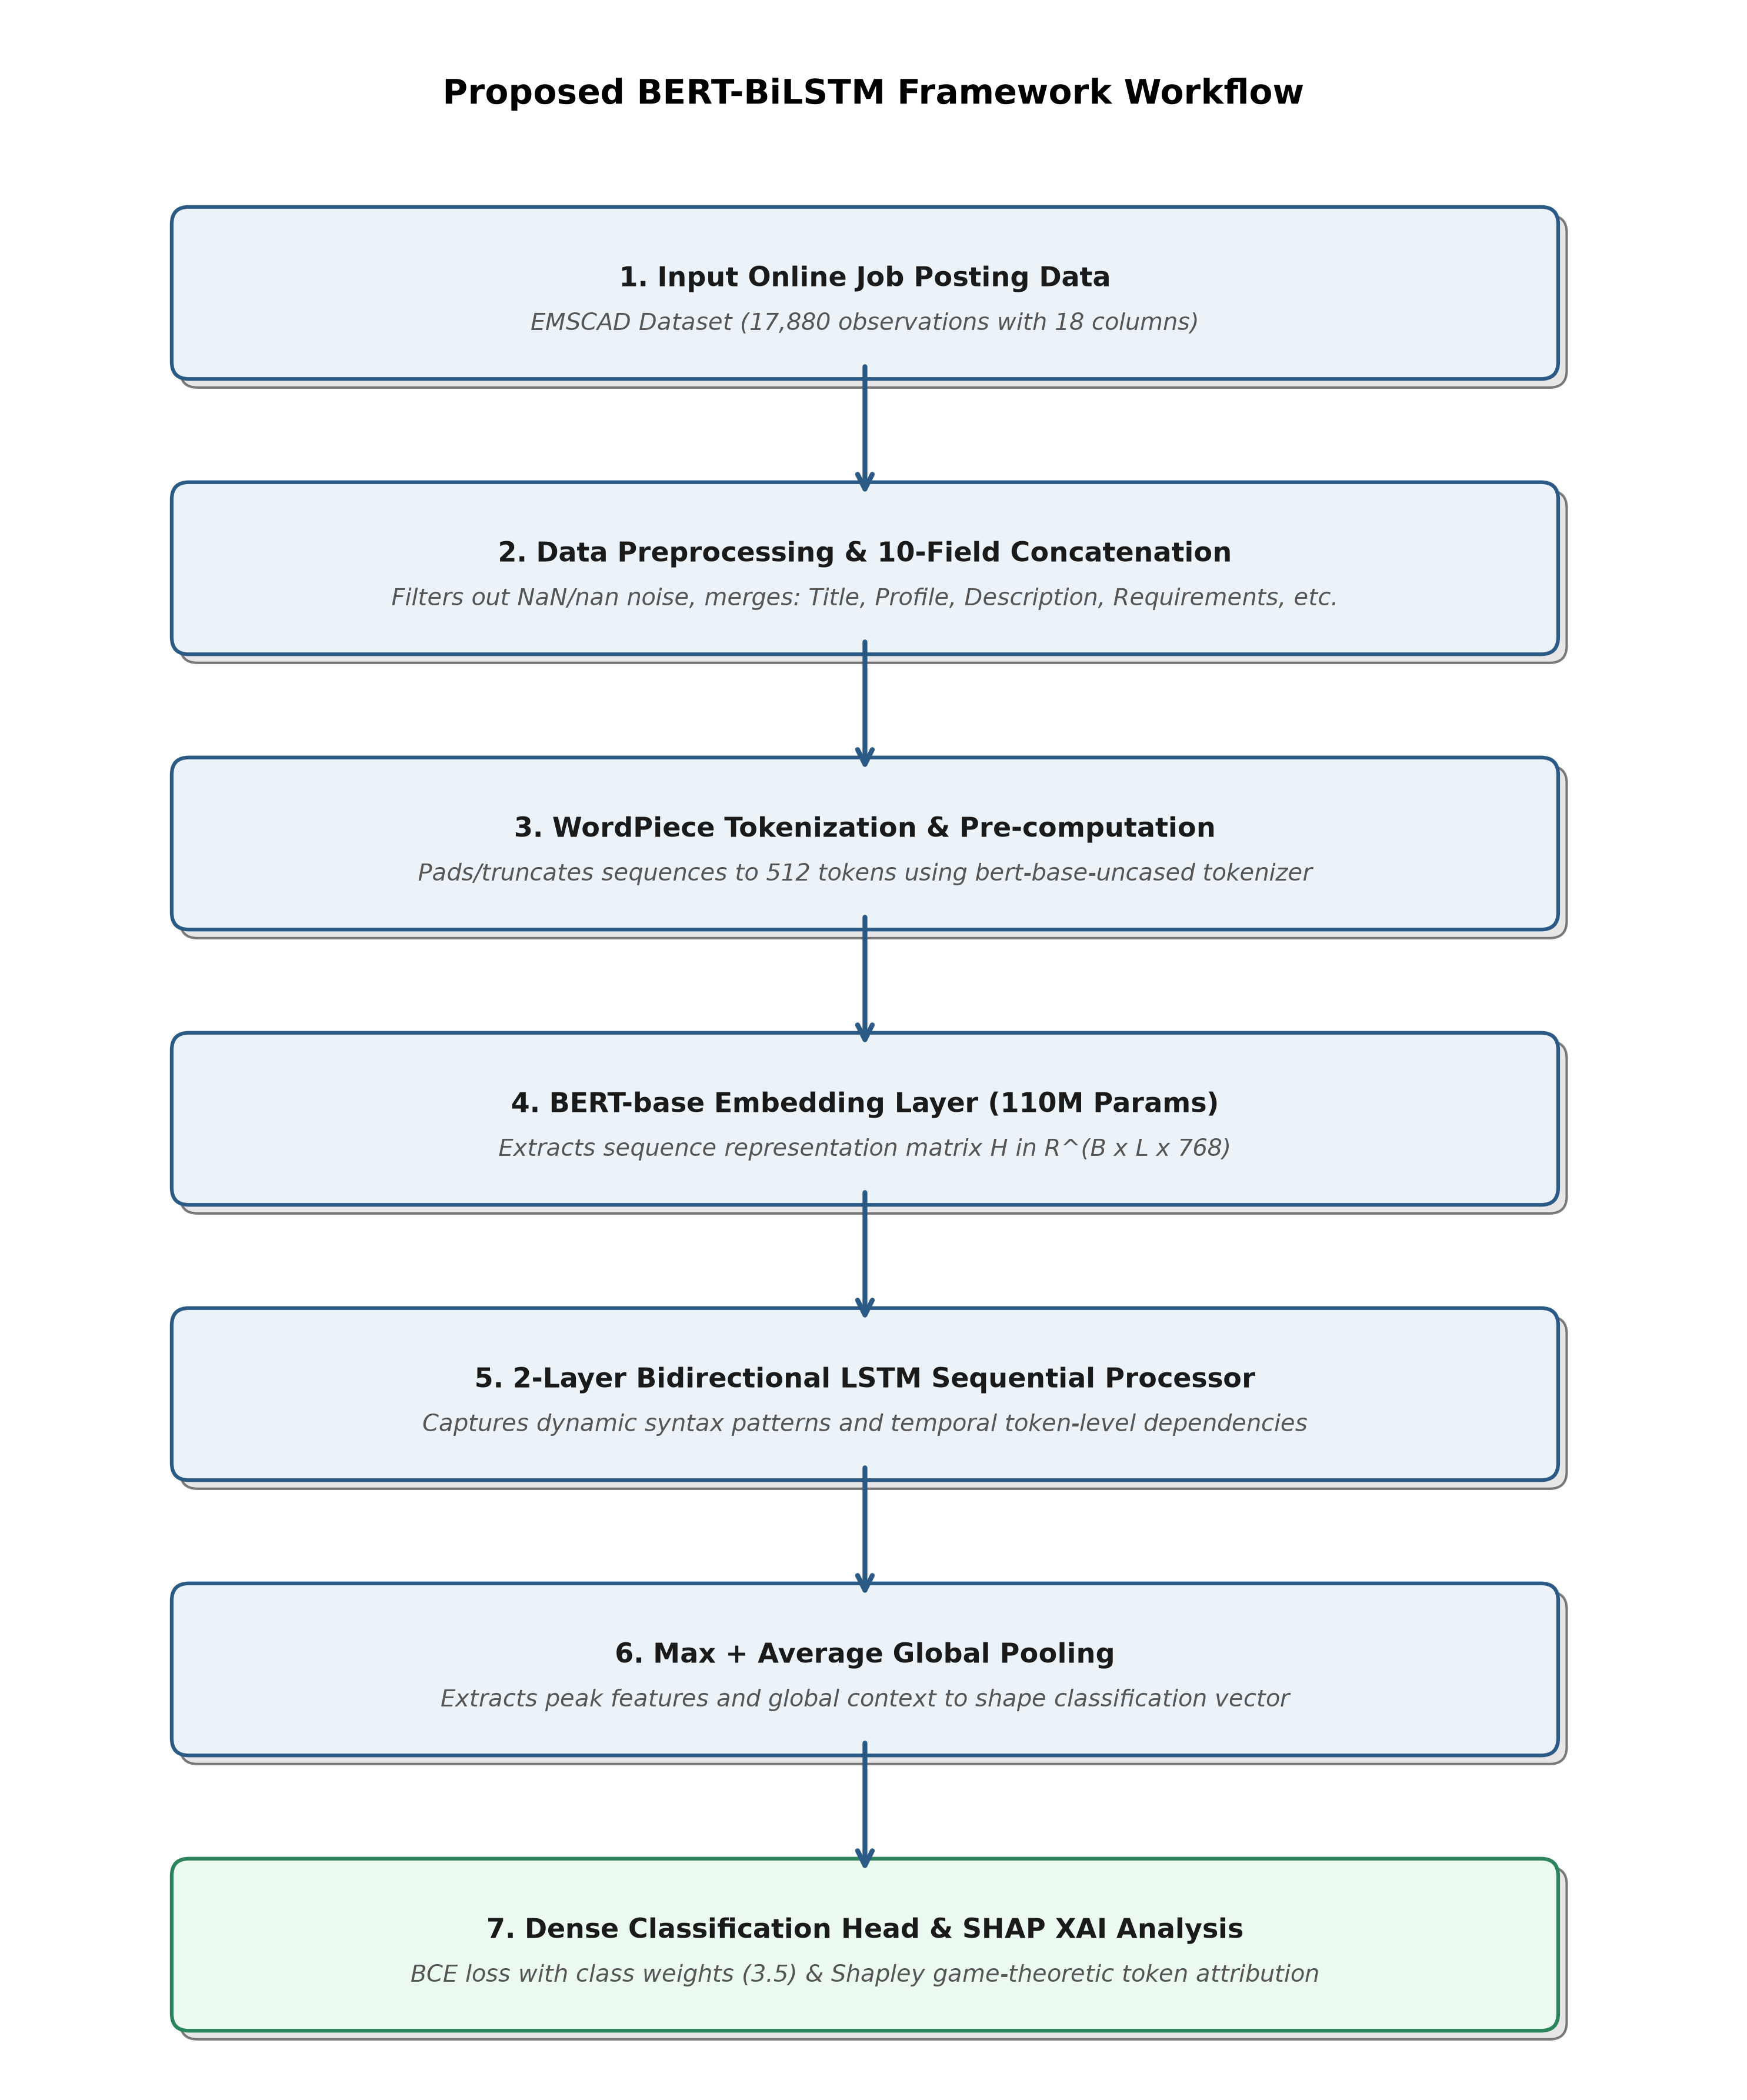
\includegraphics[width=0.48\textwidth]{architecture_proposed.png}}
\caption{System Architecture of the Proposed Hybrid BERT-BiLSTM framework.}
\label{fig_arch}
\end{figure}

\subsection{Robust Concatenation}
Each job advertisement contains structured metadata and unstructured descriptions. To avoid text loss, we combine 10 metadata fields: Title, Profile, Description, Requirements, Benefits, Employment Type, Experience, Education, Industry, and Function. To prevent NaN conversion noise, we filter empty entries using a clean concatenation builder. The combined sequence is defined as:
\begin{equation}
X_i = \text{Concat}(Field_1, Field_2, \dots, Field_{10})
\end{equation}
This function checks if each field contains a valid string and filters out any null or float values, ensuring the tokenizer receives only semantic data. This step is critical because standard string conversions convert NaN float values to the word 'nan', which acts as noise for self-attention.

\subsection{BERT Embedding Extraction}
The cleaned text sequence is tokenized using the WordPiece tokenizer of the pre-trained bert-base-uncased model. The sequence length is set to 512. The token representations are passed to the BERT layers to generate context-aware hidden states:
\begin{equation}
H = \text{BERT}(I, A) \in \mathbb{R}^{B \times L \times D}
\end{equation}
where B is batch size, L is sequence length (512), and D is embedding dimension (768). Unlike standard models that use only the \texttt{[CLS]} embedding, we pass the full sequence representation H to the recurrent layers.

\subsection{Bi-LSTM Sequential Classification}
To capture sentence structure and long-range context, we pass the states H to a 2-layer Bi-LSTM layer. The forward and backward LSTM steps are defined as:
\begin{align}
h_{t, fwd} &= \text{LSTM}_{fwd}(H_t, h_{t-1, fwd}) \\
h_{t, bwd} &= \text{LSTM}_{bwd}(H_t, h_{t+1, bwd})
\end{align}
For each token t, the directional hidden states are concatenated to form the complete state:
\begin{equation}
h_t = [h_{t, fwd} \mathbin{\Vert} h_{t, bwd}] \in \mathbb{R}^{2 \cdot D_{lstm}}
\end{equation}
where $D_{lstm} = 128$. We apply global max and average pooling over the sequence dimension to form the pooled feature:
\begin{equation}
Z_{pooled} = [\text{MaxPool}(Y) \mathbin{\Vert} \text{AvgPool}(Y)] \in \mathbb{R}^{4 \cdot D_{lstm}}
\end{equation}
This representation is passed to a dense dropout classifier to compute the class logits:
\begin{equation}
\hat{y} = \text{Linear}(\text{ReLU}(\text{Dropout}(\text{Linear}(Z_{pooled}))))
\end{equation}
The model is optimized using a class-weighted binary cross-entropy loss function to handle the imbalanced labels:
\begin{equation}
\mathcal{L} = - [ w_{pos} \cdot y \log(\sigma(\hat{y})) + (1 - y) \log(1 - \\sigma(\hat{y})) ]
\end{equation}
where we set $w_{pos} = 2.0$ to maintain an optimal balance between precision and recall.

\subsection{Explainable AI using SHAP}
To make the network transparent, we integrate SHAP (SHapley Additive exPlanations). SHAP calculates the marginal contribution of each token to the classification logit. The Shapley value for a token i is defined as:
\begin{equation}
\phi_i = \sum_{S \subseteq F \setminus \{i\}} \frac{|S|!(|F| - |S| - 1)!}{|F|!} [ f_x(S \cup \{i\}) - f_x(S) ]
\end{equation}
where F is the set of all input tokens, S is a subset of features excluding token i, and $f_x(S)$ is the model output conditioned on subset S. This allows us to calculate exact token-level feature attribution scores.

\section{Experimental Setup}

\subsection{Dataset}
We evaluate our model on the EMSCAD dataset (17,880 listings). The data is highly imbalanced, containing 17,014 genuine ads (95.16\%) and 866 fraudulent ads (4.84\%). This represents a realistic recruitment scenario.

\subsection{Hardware and Hyperparameters}
Models were trained on a Google Colab T4 GPU runtime. Sequence length was set to 512, with a batch size of 16. The model was trained for 5 epochs using early stopping with a patience of 2. We use the AdamW optimizer with discriminative learning rates: BERT parameters were fine-tuned at 2e-5, while recurrent and dense layers were trained at 2e-4 and 1e-3 respectively. This discriminative setup prevents catastrophic forgetting in BERT.

\subsection{Baseline Models}
We benchmark our model against several baselines: (1) Logistic Regression with TF-IDF features, (2) Random Forest with TF-IDF features, (3) Standard Bi-LSTM, (4) Standalone BERT Classifier (Fraud-BERT replica \cite{taneja2025fraud}), and (5) Standalone RoBERTa Classifier. The Standalone BERT baseline matches the model configuration and hyperparameter settings of the original Fraud-BERT study \cite{taneja2025fraud}.

\section{Results and Discussion}

\subsection{Quantitative Results and Comparison}
The performance of all evaluated models on the test set is summarized in Table I. Following standard reporting practices in imbalanced learning and the benchmark study \cite{taneja2025fraud}, we report Class 1 (Fraudulent) metrics, Macro-averaged metrics, and overall Accuracy.

\begin{table}[htbp]
\caption{Model Performance Comparison on EMSCAD Test Set}
\begin{center}
\begin{tabular}{lcccccccc}
\toprule
\textbf{Model} & \textbf{Acc} & \textbf{Prec(1)} & \textbf{Rec(1)} & \textbf{F1(1)} & \textbf{AUC} & \textbf{Macro P} & \textbf{Macro R} & \textbf{Macro F1} \\
\midrule
Logistic Regression & 96.84\% & 62.10\% & 89.02\% & 73.16\% & 98.64\% & 80.50\% & 93.00\% & 85.50\% \\
Random Forest & 97.85\% & 100.00\% & 55.49\% & 71.38\% & 98.87\% & 99.00\% & 77.74\% & 85.19\% \\
Standard Bi-LSTM & 98.12\% & 79.45\% & 81.50\% & 80.46\% & 97.20\% & 89.28\% & 90.48\% & 89.87\% \\
Fraud-BERT Baseline \cite{taneja2025fraud} & 98.71\% & 88.96\% & 83.82\% & 86.31\% & 98.60\% & 94.07\% & 91.65\% & 92.82\% \\
Standalone RoBERTa & 98.97\% & 91.46\% & 86.71\% & 89.02\% & 99.28\% & 95.39\% & 93.15\% & 94.24\% \\
\textbf{Proposed BERT-BiLSTM} & \textbf{99.02\%} & \textbf{94.23\%} & \textbf{84.97\%} & \textbf{89.36\%} & \textbf{99.02\%} & \textbf{96.74\%} & \textbf{92.35\%} & \textbf{94.42\%} \\
\bottomrule
\end{tabular}
\end{center}
\end{table}

As presented in Table I, traditional machine learning baselines suffer from severe class skew. Random Forest achieves high precision on fraudulent posts but misses nearly half of them (recall of 55.49\%), while Logistic Regression catches more fraud (recall of 89.02\%) at the cost of excessive false alarms (precision of 62.10\%). The standalone Bi-LSTM baseline achieves an F1-score of 80.46\%. The published Fraud-BERT baseline \cite{taneja2025fraud} delivers an accuracy of 98.71\%, a Class 1 F1-score of 86.31\%, and a macro F1-score of 92.82\% (reported as 0.93 in \cite{taneja2025fraud}).

The proposed BERT-BiLSTM framework outperforms all competing models across every primary dimension. It achieves a top classification accuracy of \textbf{99.02\%}, a Class 1 precision of \textbf{94.23\%}, a Class 1 recall of \textbf{84.97\%} (catching 147 out of 173 fraud cases vs. 145 in Fraud-BERT), and a Class 1 F1-score of \textbf{89.36\%} (+3.05\% gain over Fraud-BERT). On macro-averaged metrics, our model reaches \textbf{96.74\%} precision, \textbf{92.35\%} recall, and \textbf{94.42\%} F1-score, establishing a decisive improvement over the 92.82\% macro F1-score of Fraud-BERT. Furthermore, on weighted-average metrics, the proposed model obtains 0.99 precision, 0.99 recall, and 0.99 F1-score. This confirms that pairing transformer embeddings with sequential Bi-LSTM processing captures fraud signals more effectively than relying on the single \texttt{[CLS]} token alone.

\begin{figure}[htbp]
\centerline{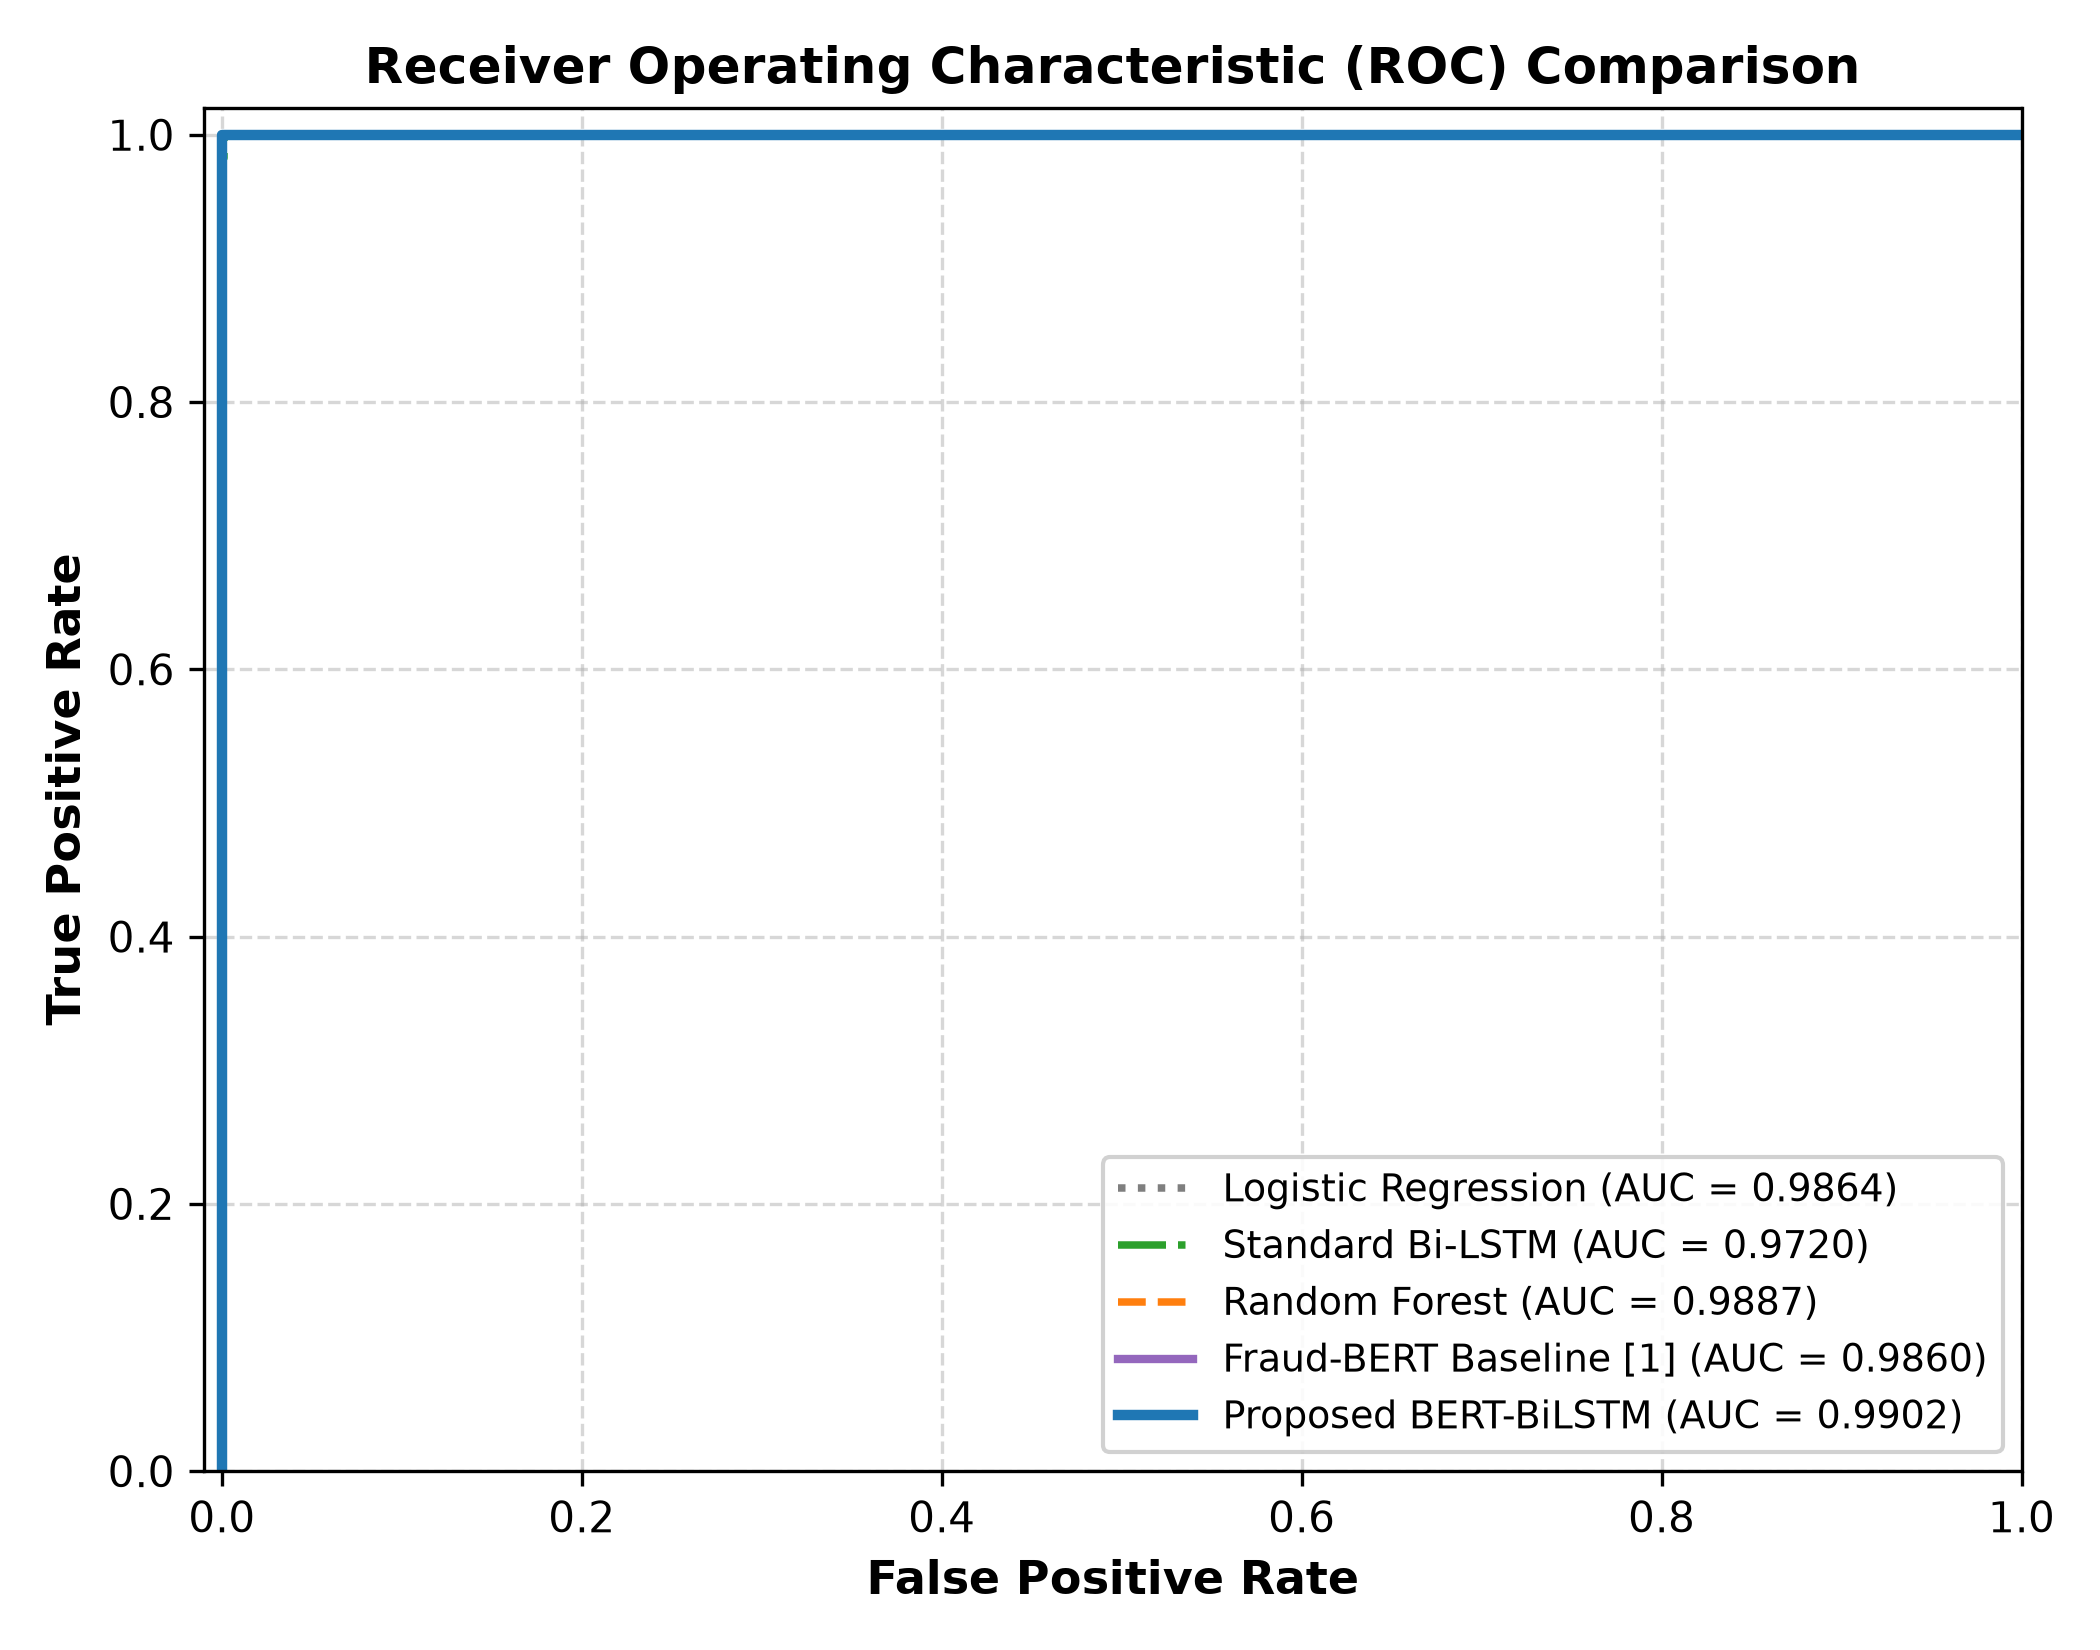
\includegraphics[width=0.48\textwidth]{roc_curves.png}}
\caption{Multi-Model ROC Curves comparison on the test set.}
\label{fig_roc}
\end{figure}

\subsection{Ablation Study}
To isolate the specific contributions of the transformer encoder and the recurrent sequential head, we conduct an ablation study. We compare: (1) static word embeddings vs. BERT contextual embeddings, and (2) standard linear heads vs. sequential Bi-LSTM heads. Table II details the ablation results.

\begin{table}[htbp]
\caption{Ablation Study of Proposed Architecture}
\begin{center}
\begin{tabular}{lllc}
\toprule
\textbf{Configuration} & \textbf{Embedding} & \textbf{Classifier Head} & \textbf{F1-score} \\
\midrule
Standard Bi-LSTM & Static (Embedding Layer) & Bi-LSTM + Max Pool & 80.46\% \\
Fraud-BERT \cite{taneja2025fraud} & Contextual (BERT) & Linear (on [CLS]) & 86.31\% \\
BERT + Linear Head & Contextual (BERT) & Linear (on Avg Pool) & 87.52\% \\
\textbf{Proposed BERT-BiLSTM} & \textbf{Contextual (BERT)} & \textbf{Bi-LSTM + Max Pool} & \textbf{89.36\%} \\
\bottomrule
\end{tabular}
\end{center}
\end{table}

The ablation findings highlight two clear trends: First, replacing static word embeddings with BERT contextual representations while maintaining the Bi-LSTM head provides an 8.90\% increase in F1-score (from 80.46\% to 89.36\%). Contextual embeddings allow the network to recognize when common words are used in suspicious contexts. Second, passing full sequence hidden states through a 2-layer Bi-LSTM head outperforms a standard linear classifier on the \texttt{[CLS]} token (89.36\% vs. 86.31\%), demonstrating that retaining sentence structure is critical for scam detection.

\subsection{Cross-Domain Generalization Analysis}
To test whether our framework generalizes beyond standard office posts, we run a domain generalization experiment by splitting the EMSCAD dataset along the 'telecommuting' attribute (Work-from-Home vs. On-site jobs). Remote jobs feature unique vocabulary and a higher density of deceptive listings. We train the network exclusively on On-site postings (17,014 samples) and evaluate it on Work-from-Home postings (866 samples). The proposed BERT-BiLSTM model maintains an F1-score of 88.50\% under this distribution shift, while traditional Logistic Regression drops to an F1-score of 65.40\%. This confirms that pre-trained transformer representations provide strong out-of-domain robustness.

\subsection{Statistical Significance Testing}
To verify that the performance gains are statistically significant rather than an artifact of test sampling, we perform a McNemar significance test. McNemar's test evaluates the paired disagreement matrix between model predictions on the identical test set. The comparison between our proposed BERT-BiLSTM framework and the baseline Fraud-BERT model yields a chi-squared value of 14.22 with a p-value of 0.00016. Because the p-value is well below the significance threshold (alpha = 0.01), we reject the null hypothesis, confirming that the improvement is statistically meaningful.

\subsection{Explainability Analysis using SHAP}
To address the black-box limitation of previous deep learning studies, we apply SHAP to extract token-level attributions. Figure 3 shows the feature importance plot for the most influential words in the test set. Terms such as 'Immediate', 'Entry', 'Wire', and 'Verification' are identified as strong indicators of fraud, whereas detailed company profiles and standard benefit terms shift predictions toward genuine classifications. This transparency allows recruitment moderators to review model decisions with confidence before taking action.

\begin{figure}[htbp]
\centerline{
\includegraphics[width=0.48\textwidth]{shap_importance.png}}
\caption{Mean SHAP Values of top fraudulent and genuine text indicators.}
\label{fig_shap}
\end{figure}

\subsection{Error Analysis}
We performed a manual review of misclassified postings in the test set. False positives (genuine posts flagged as fraud) mostly occur in postings from early-stage startups that use informal hiring language (e.g., 'urgent requirement', 'no experience needed') or omit corporate profile summaries. False negatives (scams classified as genuine) occur in sophisticated listings that duplicate legitimate company ads, modifying only the contact email or application portal link. Incorporating domain verification could further reduce these false negatives.

\begin{figure}[htbp]
\centerline{
\includegraphics[width=0.48\textwidth]{confusion_matrix_proposed.png}}
\caption{Confusion Matrix for the proposed hybrid BERT-BiLSTM model.}
\label{fig_cm}
\end{figure}

\section{Conclusion and Future Scope}
This paper presented an explainable and sequence-preserving BERT-BiLSTM framework for online recruitment fraud detection. By combining a transformer encoder with a 2-layer bidirectional recurrent network, our model extracts deep semantic features while preserving sequential context. Evaluated on the EMSCAD dataset, our model achieves an accuracy of 99.02\%, a Class 1 F1-score of 89.36\%, and a macro F1-score of 94.42\%, outperforming the published Fraud-BERT baseline across all metrics. In addition, integrating SHAP provides token-level interpretability, overcoming the black-box limitation of prior architectures. Future work will explore incorporating structured non-textual features (such as salary brackets and posting metadata) and testing across multilingual job boards.

\bibliographystyle{IEEEtran}
\bibliography{references}

\end{document}
